%--------------------------------------||--------------------------------------%

\documentclass[11pt,letterpaper]{article} %  font size


%-----------------------------------PACKAGES-----------------------------------%

\usepackage[T1]{fontenc} % Choose an output font encoding (T1) that has support for the accented characters used by the most widespread European languages
\usepackage[utf8]{inputenc} % Allow input of accented characters (and more...)
\usepackage{textcomp,marvosym} % additional figures, including textdegree
\usepackage{graphicx} %  figures
\usepackage[round]{natbib} % names in citations
\usepackage{lineno} % line numbers
\usepackage{authblk} % allows more intuitive formatting for multiple authors/affiliations
\usepackage[margin=1in]{geometry} % make the margins 1 inch on all sides of the document
%\usepackage{amsmath} % useful for formatting math stuff, especially complex equations
%\usepackage{pdflscape} % rotate table into landscape mode
%\usepackage{subfigure} % side by side figures
%\usepackage{longtable} % for tables that span multiple pages.
\usepackage{setspace} % double spacing



%----------------------------------FORMATTING-----------------------------------

%\topmargin -1cm %0.0cm
%\textwidth 16cm % what does this do?
%\textheight 21cm % what does this do?
%\footskip 1.0cm % what does this do?
%\oddsidemargin 0.0cm

\date{\today}
\doublespacing % initiate double spacing (package setspace)
%\linespread{2} % alternate method of double spacing
%\graphicspath{{../../Figures/}} % I think if you do this it saves typing the path over and over in the figures section


%------------------------------------TITLE--------------------------------------

\title{There once was a grid at ol' Carkeek}

%-----------------------------------AUTHORS-------------------------------------

% using package 'authblk':
\author[1]{First Author\thanks{first.author@funstuff.com}}

\author[1,2]{Second Author}

\author[2]{Third Author}

\affil[1]{Department of Computer Science, \LaTeX\ University}
\affil[2]{Department of Mechanical Engineering, Superfabulous University}



%----------------------------------FORMATTING-----------------------------------
\begin{document}
\maketitle
\linenumbers % start line numbers
\def\linenumberfont{\normalfont\small\rmfamily} % change line number font


%----------------------------------KEYWORDS-------------------------------------
\section*{Keywords}
Stuff, things, neat, cool, wow, instafun, tags4likes, etc

%----------------------------------ABSTRACT-------------------------------------
\section*{Abstract}
This is the text of the abstract.

%---------------------------------INTRODUCTION----------------------------------
\section*{Introduction}

Biodiversity surveillance is being revolutionized by DNA-based detection of organisms from environmental samples. ?(specifically speed and scope of ecological studies).
Many researchers are justifiably cautious about the ?(adoption) of this new form of data.
Their apprehension is rooted in the premise that traditional survey approaches are more accurate because the chain of inference between observation and ecological data is usually short: A researcher sees two swans in Lake Hopatcong and infers the lake is occupied by at least 2 swans.
DNA based surveys, on the other hand, consist of a longer chain of inference:
DNA sequences are reported by a sequencing machine, the machine identifies the sequence of products of a polymerase chain reaction (PCR), PCR amplifies pieces of DNA from a purified genomic DNA sample, DNA is purified (extracted) from an environmental sample, environmental samples contain DNA from organisms present, the organisms present are representative of the biological community about which we wish to make inference. ?( reverse order? tie to concrete example (swans of Lake Hopatcong)).
Clearly, this process is more complex than visual surveys, as the relationship between several steps is complex or unknown.
But consider that the processes ?(behind | underlying) other more widely-used ecological survey techniques are similarly complex, such as bird surveys based on song, or visual identification of fungal spores. When alternate survey approaches are impossible or inefficient, we are more willing to accept any available survey data, regardless of the complexity or uncertainty underlying it. (microbiologists have enthusiastically relied on DNA-based surveys for years for this reason, (though yes, they also do not have the problem of disconnect between individual and cell)).

The ability of DNA surveys to make quantitative inference about communities has been touted by some (CITE new fish quantitation paper) and doubted by others (CITE european eelgrass PLOSONE).
For example, a study linking (blah blah blah) concluded that "metabarcoding is powerful, yet blind" (CITE european eelgrass).
Conversely, others have reported strong quantitative and intuitive links between DNA-based and traditional survey methods (CITE Port 2016 MOLECO).
These studies usually rely on simple statistical models to link DNA quantity to some measurable ecosystem property like biomass (but see CITE).
When confronted with data collected in ?(complex ways/studies/whatever), simple models ?(may | often) fail to detect relationships when they exist, or vice versa ?(they are prone to inflated risk of BOTH type I and type II error) (CITE, see Woltman 2012).
For example, (CITE, look for that Gelman paper) have demonstrated that when data are structured in a hierarchical fashion (e.g. test scores of students in schools belonging to districts belonging to states), a low number of replicates at the first level of hierarchy (SEE THE PAPER).
Similarly, (describe hospital/school problems).

Shelton et al. (CITE Shelton 2016) outlined an approach for structuring statistical models of DNA surveys that address these issues.
This framework improved on alternative statistical techniques by explicitly accounting for the ?(hierarchical | nested | multilevel) structure of the study design, which allows error and uncertainty at each level to be ?(explicitly accounted for| modeled | propagated throughout the model).
That study demonstrated an improvement in the estimate of higher-level (e.g. ecological community) quantities when the processes linking them to the data are specified.
As an example, it was shown that incorporation of data about the mismatch between primer and template DNA sequence can improve the estimate of the relative abundance of unique DNA templates input to a PCR.

Here, we apply this framework to a DNA survey of ?(nearshore | coastal) marine habitat.
(TODO add commentary on current dogma surrounding distribution of DNA in well-mixed (marine) habitats).
We document the variability associated with lab based ?(procedures | replication | treatment; i.e. filter+DNA+PCR+seq), and the spatial scale over which DNA communities vary in this habitat.
We ?(show that | tested whether) a taxon's spatial distribution predicts ( the slope of the relationship between distance from shore and DNA abundance ~or~ to what degree DNA abundance is explained by distance from shore for each taxon).
We focus partly on species with known life histories that define their spatial distribution (e.g. shallow water livebearing fishes or sessile intertidal organisms with ?(motile/planktonic/pelagic) larvae or gametes).
For these taxa whose spatial distribution is well-documented and restricted, we calculate the rate of change in space and compare this rate among taxa with similar spatial distributions.
In turn, the distribution of rate of change serves as an estimate of the spatial distribution of DNA in this habitat.

We would love to estimate the minimum distance over which eDNA community differences can be detected.

% We measure 'extra-(corporeal|organismal) DNA
Some authors have cautioned against the use of DNA-based macrobial communities in marine environments because they are subject to dynamic physical forces (CITE).
If environmental circulation 
In general, the relationship between community dissimilarity (0 = identical; 1 = completely different) and spatial distance is expected to be asymptotic, because communities nearer to each other tend to be more similar than those farther apart.
The intercept is expected to be near 0, because samples taken at the same place should be very similar. % technically impossible for samples to be taken at exactly 0; they are actually immediately adjacent.
Deviation in the intercept from 0 indicates heterogeneous community composition/structure over fine scales.
A flat relationship between dissimilarity and distance indicates that heterogeneity is not assorted spatially, and can be interpreted in different ways, depending on the mean.
If the mean is near 1, the spatial heterogeneity has overwhelmed the spatial scale of sampling.
If the mean is near 0, there is no community heterogeneity over the scale sampled.


%-----------------------------------METHODS-------------------------------------
\section*{Methods}
\subsection*{Environmental Sampling}
Starting from lower-intertidal patches of \textit{Zostera marina}, we collected water samples at 1 meter depth from 8 points (0, 75, 125, 250, 500, 1000, 2000, and 4000 meters) along three parallel transects separated by 1000 meters (Figure \ref{site_map}).

\subsection*{Laboratory Methods}

Samples were randomly assigned to PCR primer and library adapter index sequences.
The sequencing run consisted of 14 samples ('libraries') prepared using different index sequences ligated during library preparation.
Of these libraries, ten comprised of amplicons prepared using the 16S protocol reported above, and four comprised of amplicons prepared using a 12S protocol similar to that reported by (CITE PORT 2015).

Pooled libraries were sequenced on the Illumina NextSeq platform at the Stanford Center for Functional Genomics (machine ID: NS50061; run ID: 115; flowcell ID: H3LFLAFXX). Raw sequence data in fastq format is publicly available (see Data Availability).

\subsection*{Data Preparation (Bioinformatics)}
Detailed bioinformatic methods are provided in the supplemental material, and scripts used from raw sequencer output onward can be found in the project directory on GitHub (see Data Availability).



%----------------------------------------------------------------------------
%METHODS
%Sequences passing were demultiplexed on the basis of the ?(8-bp) sequence ligated during library preparation and read during the index read, and filtered for general quality by the sequencing facility.
%
%We used fastqc to assess the fastq files output from the sequencer for low-quality indications of a problematic run.
%
%Reads that contain primer index sequences (or combinations thereof) that we did not actually use in laboratory procedures are known to ?(be derived from contamination) be a result of processes that leave the same signature as contamination. For example, errors during oligonucleotide synthesis of the indexed primers would cause reads to be erroneously assigned to samples.
%Because this represents the minimum rate at which we can be certain that sequences from one environmental sample could be erroneously assigned, we considered for further analysis only those reads occurring with greater frequency than this.
%
We calculated rates of cross-library contamination by counting occurrences of primer sequences: 12S primer sequences appearing in a 16S library (and vice versa) indicate an error in the preparation or sequencing procedures.

We assessed PCR contamination by evaluating the dissimilarity of replicate PCRs of the same DNA sample, and removed one sample for which the Bray-Curtis dissimilarities between itself and the other replicates exceeded 0.1 (lib\_B\_tag\_GCGCTC).

%To infer a general estimate of the rate of cross-sample contamination likely to be associated with lab procedures, we calculated the proportion of reads containing primer index sequences (or combinations thereof?) that we did not actually use
%
%RESULTS
%Reads were of generally high-quality, with ?(96.48)? % of base calls having a 0.001 or lower probability of incorrect base call (Phred q-score of 30 or higher).
%
%
%Total sequencing clusters passing filter per read: 371,576,190 on NEXTSEQ
%
% THESE BELOW ARE FROM A MISEQ RUN
%reads, reads passing filter, % >= Q30, for each run ( 7,052,307 ; 6,752,829; 97.47 :: 7,052,307 ; 6,752,829 ; 95.50)
%
%Cluster density of 358 \UTF{00EF}\UTF{00BF}\UTF{0153}22	clusters per mm^2
%
%XXX % of reads aligned to the PhiX genome
%(31.02 \UTF{00EF}\UTF{00BF}\UTF{0153}0.59	; 29.17 \UTF{00EF}\UTF{00BF}\UTF{0153}0.89)
%
%and error rate as determined from alignment of PhiX reads to the PhiX genome was low (Read 1: 1.26 \UTF{00EF}\UTF{00BF}\UTF{0153}0.07; Read 2: 1.38 \UTF{00EF}\UTF{00BF}\UTF{0153}0.07)
%----------------------------------------------------------------------------


To scale the OTU counts, we calculated the minimum number of OTU-assigned reads (as opposed to raw number of reads) found in these samples (130402), multiplied this by within-sample proportional abundance of each OTU, and finally rounded these numbers.




\subsection*{Community Analysis}

We subset the data in a variety of ways and conducted each analysis on all subsets.
We report the subset used with each analysis, and report results on alternative subsets in the supplemental material. 
For all analyses beyond the assessment of PCR consistency, we use the mean taxon abundance across PCR replicates from each of the 24 environmental samples.
Our subsetting methods were (1) exclude rare taxa ?(threshold)?, (2) exclude abundant taxa ?(threshold)?, (3) subsampling of taxa randomly, (4) subsampling of taxa proportional to their abundance, (5) subsampling of taxa inversely proportional to their abundance, (6) exclude taxa found in only one environmental sample (spatially invariant), (7) exclude non-marine taxa (e.g. humans, pigs), (8) exclude taxa whose known individual range (including gametes and larvae) exceeds the spatial scale of our study. 
We also tested a variety of transformations of the mean scaled abundance data, including (1) log ($log_{e}x$), and (2) binary ($1 = x > 1$; $0 = x < 1$).

% Used k-medoids (PAM) rather than k-means because it does not require euclidean distances can be computed and that the observations follow a gaussian distribution
% because of the nature of our data (lots of zeros, with some very high counts), the mean is not very informative
We simultaneously assessed the existence of distinct community types and the membership of samples to those community types using a partitioning around mediods algorithm (CITE PAM, sometimes referred to as k-medoids clustering), as implemented in the R package fpc (CITE fpc).
The classification of samples to communities was made on the basis of their pairwise Bray-Curtis dissimilarity, calculated using the function vegdist in the R package vegan (CITE VEGAN). % consider Gower distance

We calculated the great circle distance between points using the Haversine method as implemented by the R package geosphere (CITE geosphere).
% Calculate Moran's I on ?(relative abundance | raw count) of ?(taxa | OTU | uniq_sequences) to report dispersion of DNA in space?

\subsection*{Spatial Model Formulation}
We use the general framework outlined by Shelton et al (CITE).
That study outlined the structure for estimation of the proportional biomass of a taxon ($B_i$) given the proportional counts of sequences recovered from a parallel sequencing run ($Z_i$).

We modeled the counts of DNA sequences ($Z$) from each of a given taxon $i$, in each replicate PCR $j$, from each replicate of a given location $k$ (hence, $Z_{ijk}$), as though they are ?(proportional to/drawn from)? a Poisson distribution. A Poisson distribution is described by one and only one parameter, $\lambda$, which is equal to both the mean and variance. Because in this case our modeled values are discrete counts, we use the natural exponent, $e^\lambda$. % WHY IS IT EXPONENTIATED? COUNTS?
Thus,
\begin{equation}\label{some_cool_eqn_name}
	Z_{ijk} \sim Poisson(e^{\lambda_{ijk}})
\end{equation}

In turn, we further assume this parameter $\lambda$ is linearly proportional to a suite of taxon-, pcr-, and site- specific parameters describing the variance associated with each sub-process linking the amount of DNA ($Y$) of a given taxon $i$ at a given location $k$ in a DNA extract (hence $Y_{ik}$):

\begin{equation}\label{GLM}
	\lambda_{ijk} = \beta_0 + \beta_i + \eta_{ijk} + \epsilon_{ijk}
\end{equation}

%(\ref{my_equation_label})
Where $\beta_0$ is a general intercept across all taxa, $\beta_i$ is a fixed effect accounting for the variance associated with taxon $i$, and $\eta_{ijk}$ and $\epsilon_{ijk}$ are random effects of variance resulting from the processes associated with PCR and spatial location, respectively.



%We constructed the following mathematical model (\ref{my_equation_label}) to better understand the concept:
% using '\ref{something}' in the text will refer to any object (e.g. figure, equation, table) which contains the corresponding '\label{something}'
% Note that you need to run latex a few times to get it to register numbers correctly

%\begin{equation}\label{my_equation_label}
%	Y = 2a + 2a
%\end{equation}
%
%Where $a$ represents an apple.

%-----------------------------------RESULTS-------------------------------------
\section*{Results}
\subsection*{Data Quality (Bioinformatics)}
All value ranges are reported as (mean $\pm$ standard deviation).\\
There was a very low frequency of cross-contamination from other libraries into those reported here (5e-05$\pm$8e-05; max 0.00034)

We assessed the consistency of PCR by conducting 4 replicate PCRs for each environmental sample and calculating the mean pairwise Bray-Curtis dissimilarity of the resulting communities (scaled to minimum read depth per sample). 
92 of the 96 amplicon samples had mean Bray-Curtis dissimilarity $\leq$ 0.052; 1 sample had a value of 0.341, which elevates the value of the other replicates. 
After removal of this sample, the highest mean Bray-Curtis dissimilarity among replicates within an environmental sample was 0.034. 



\subsection*{Community Analysis}
Excluding spatially-invariant taxa ?(taxa which occur in only one spatial location) had no discernible effect on the outcome of the PAM analysis (number of clusters, assignment to clusters).

\subsection*{Spatial Model Output}


%----------------------------------DISCUSSION-----------------------------------
\section*{Discussion}
Boy those results sure are neat. Now, the pressing question becomes: How do you like them apples?

%-------------------------------ACKNOWLEDGEMENTS--------------------------------
\section*{Acknowledgements}
We wish to thank all of the little people.

%-----------------------------------FUNDING-------------------------------------
\section*{Funding}
This study was funded by our super-rich uncle.

%--------------------------------CONTRIBUTIONS----------------------------------
\section*{Author Contributions}
Conceived and designed the experiments: James L. O'Donnell, Ryan P. Kelly, A. Ole Shelton.
Collected the data: James L. O'Donnell, Greg Williams, Natalie C. Lowell, Ryan P. Kelly, A. Ole Shelton, Jameal F. Samhouri.
Conducted the analyses: .
Wrote the first draft: .
Edited the manuscript: .


%-------------------------------------DATA-------------------------------------%
\section*{Data Availablity}
% TODO SUBMIT DATA AND METADATA; ADD URL
All sequence files and metadata are available from EMBL:\\ \verb!http://www.ebi.ac.uk/ena/data/view/XXXXXXXXX! \\
All analyses were performed using scripts available from the project repository on GitHub:\\  \verb!https://github.com/jimmyodonnell/Carkeek_eDNA_grid!\\

%----------------------------------REFERENCES-----------------------------------
%\section*{References} % commented out because the section title is automatically inserted if using an automatically-generated bibliography
\bibliographystyle{apalike} % or: plain,unsrt,alpha,abbrv,acm,apalike,ieeetr
\bibliography{carkeek_grid_bib} % path to your .bib file excluding .bib extension (e.g. /Users/threeprime/Documents/Publications/bibtex/library)


%-----------------------------------FIGURES-------------------------------------
\section*{Figures}

\begin{figure}[h!] % [h!] forces the figure to be placed roughly here
  \centering
    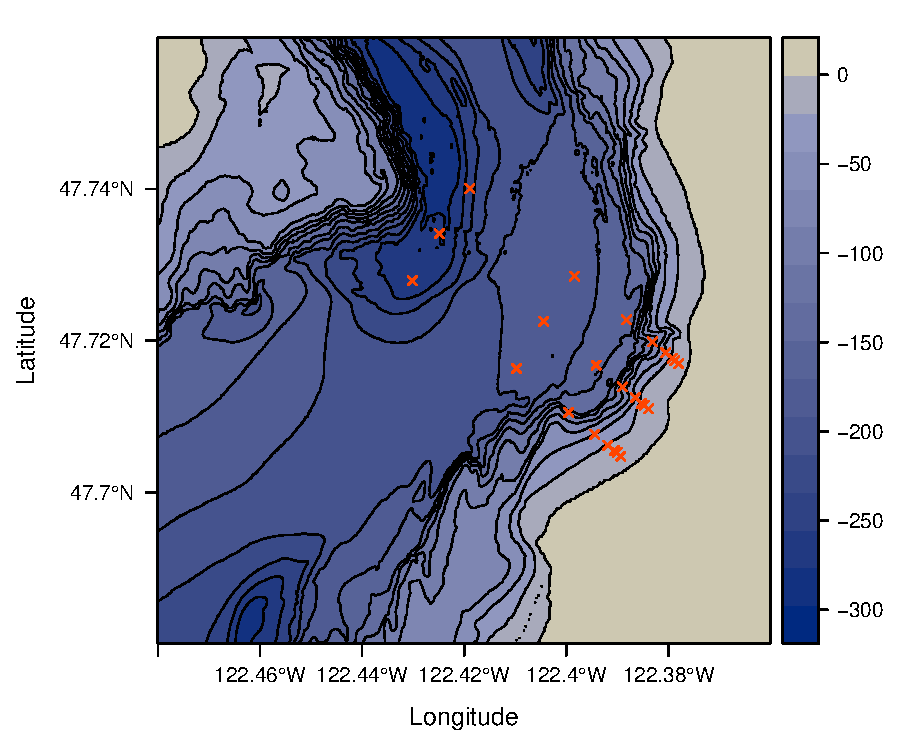
\includegraphics[width=1\textwidth]{../../Figures/site_map.pdf}
    \caption{TODO: Plot with GEBCO 30-second data or remove grid coloring and color by isobath. Looking into filling by contour. Geographic position of collected samples. Lines give XXX meter isobaths.}
  \label{site_map} % use this to refer to your figure in the text, so that numbering updates automatically
\end{figure}

\begin{figure}[h!] % [h!] forces the figure to be placed roughly here
  \centering
    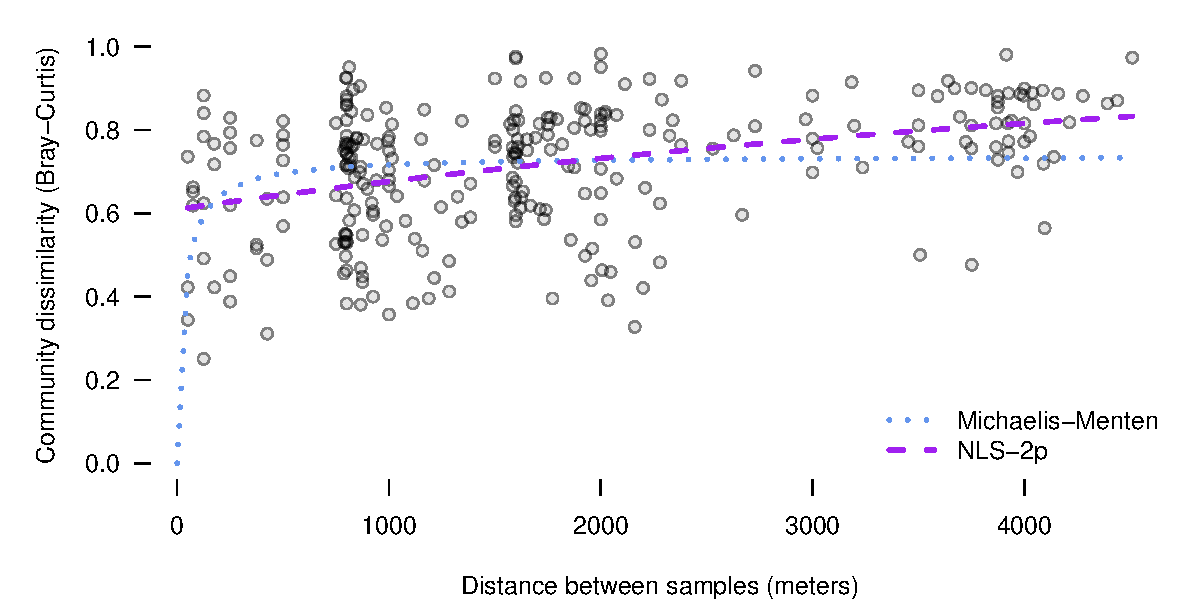
\includegraphics[width=1\textwidth]{../../Figures/diss_by_dist.pdf}
    \caption{Pairwise Bray-Curtis dissimilarity of eDNA communities plotted against pairwise spatial distance.
    Line represents prediction of Gaussian LOESS (degree = 1; span = 2/3).
    Restricting comparison to within-transect has no qualitative difference in the outcome (see 'diss\_by\_dist\_by\_transect.pdf').
    }
  \label{comm_diss_by_geo_dist} % use this to refer to your figure in the text, so that numbering updates automatically
\end{figure}


\begin{figure}[h!] % [h!] forces the figure to be placed roughly here
  \centering
    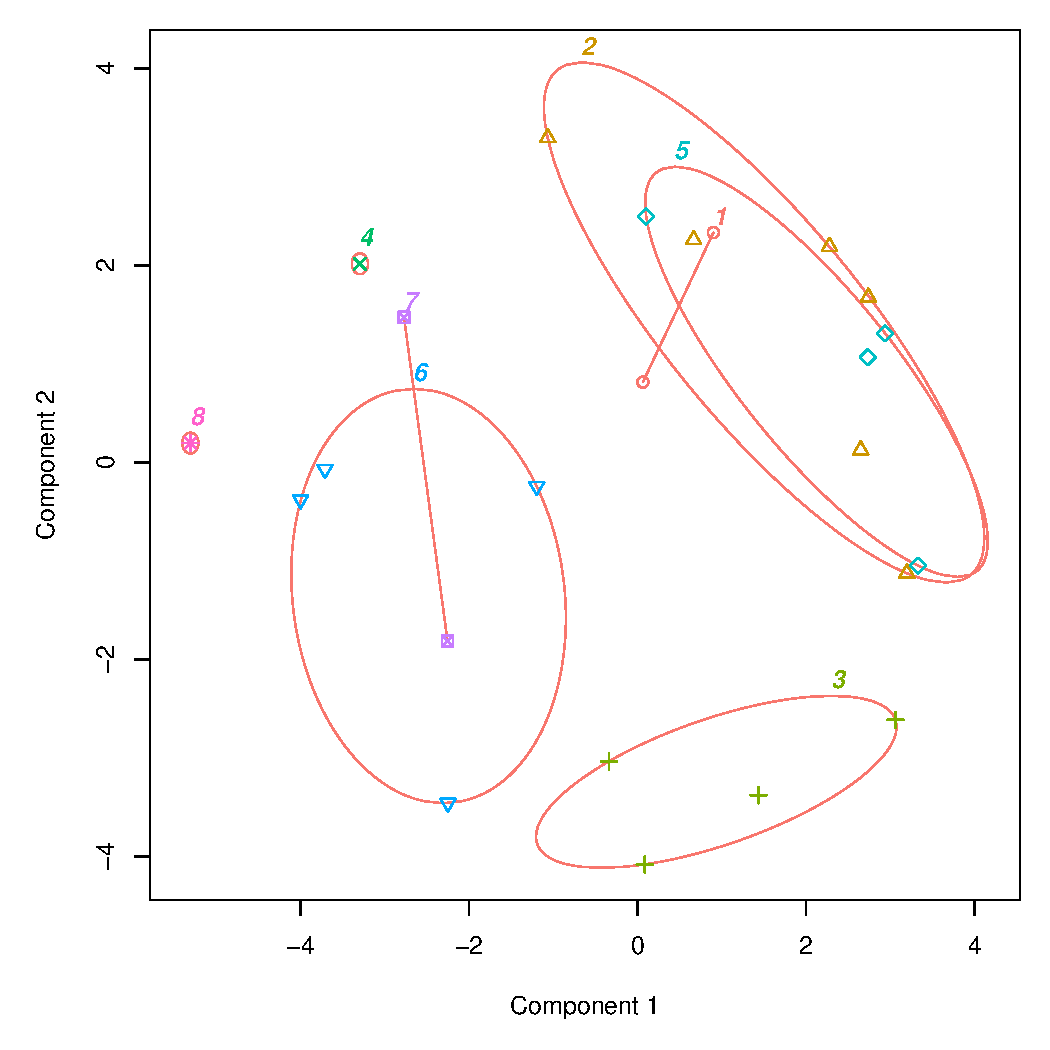
\includegraphics[width=1\textwidth]{../../Figures/pam_plot.pdf}
    \caption{TODO figure out color of ellipses; I can't even plot them gray without Plot of partitioning around medoids (PAM) analysis of OTU sequence abundance from 4 replicate PCRs at each of 24 sampling points. Points represent communities of OTUs; color and shape indicate cluster membership as determined by PAM analysis. Ellipses indicate the smallest area of a cluster that contains all of its members.}
  \label{pam_plot.pdf} % use this to refer to your figure in the text, so that numbering updates automatically
\end{figure}

\begin{figure}[h!] % [h!] forces the figure to be placed roughly here
  \centering
    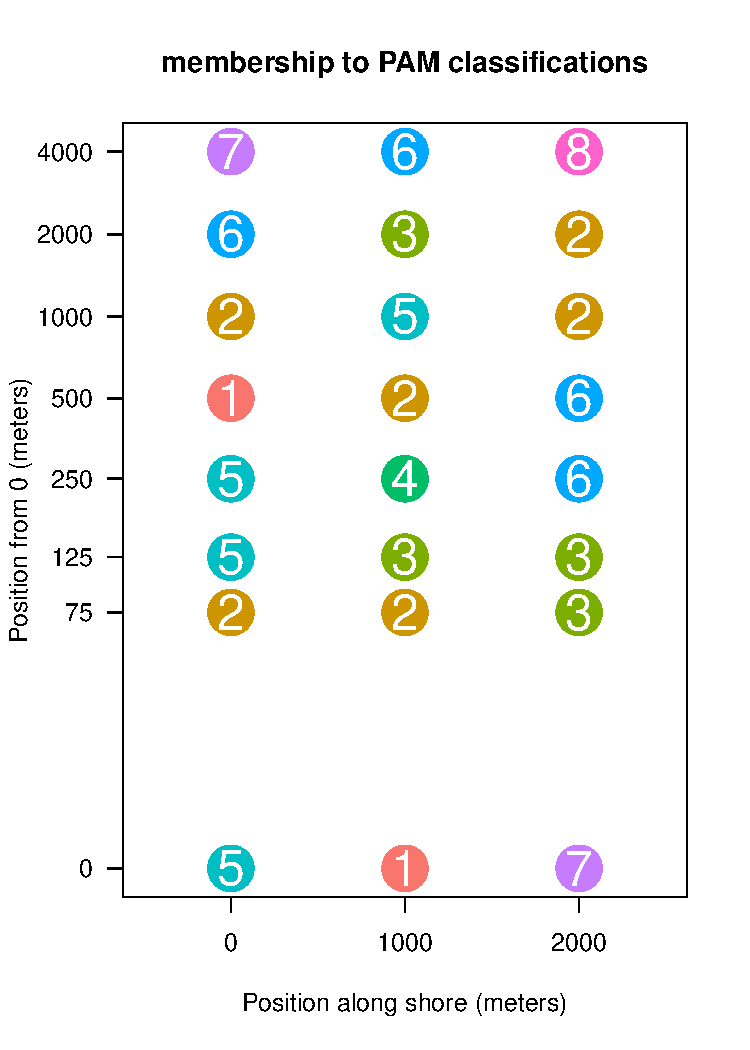
\includegraphics[width=1\textwidth]{../../Figures/pam_in_space.pdf}
    \caption{Geographic position of collected samples, colored by membership to clusters identified by partitioning around medoids algorithm. 
%    Points are jittered in both horizontal and vertical dimension to distinguish among four replicate PCR products sequenced from each environmental sample.
}
  \label{clustering_map} % use this to refer to your figure in the text, so that numbering updates automatically
\end{figure}

\begin{figure}[h!] % [h!] forces the figure to be placed roughly here
  \centering
    \includegraphics[width=1\textwidth]{../../Figures/slope_plots.pdf}
    \caption{Fit lines of DNA sequence counts as a function of distance from shore for a selection of taxa for which we have strong preconceived expectations (left). Box plots of the estimates of the slopes for taxa ?(100 most abundant)?, grouped by life history traits (right).}
  \label{slope_plots} % use this to refer to your figure in the text, so that numbering updates automatically
\end{figure}

\begin{figure}[h!] % [h!] forces the figure to be placed roughly here
  \centering
    \includegraphics[width=1\textwidth]{../../Figures/var_boxplots.pdf}
    \caption{Box plots of estimates of variance associated with each level of the multilevel model, corresponding to stages of the eDNA sampling protocol.}
  \label{variance_boxplots} % use this to refer to your figure in the text, so that numbering updates automatically
\end{figure}

\begin{figure}[h!] % [h!] forces the figure to be placed roughly here
  \centering
    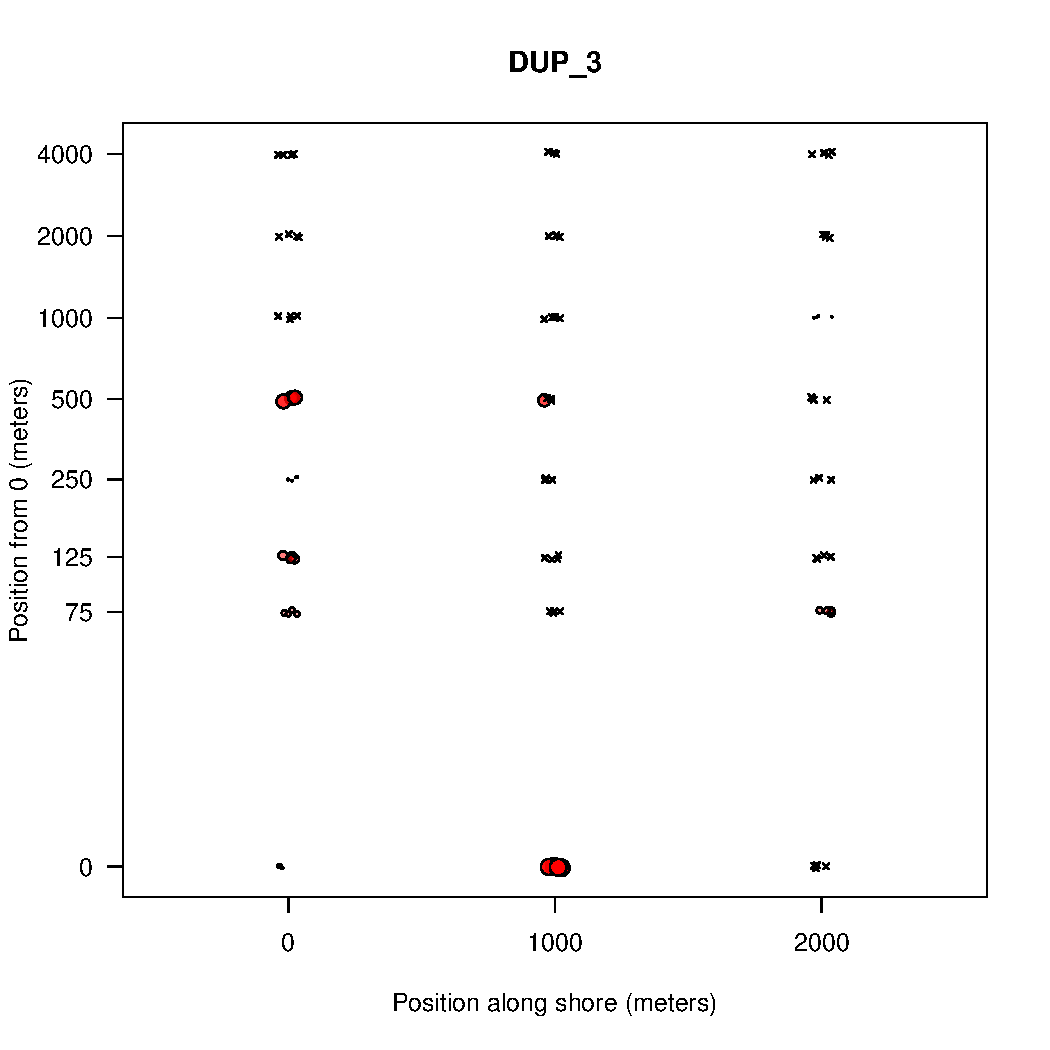
\includegraphics[width=1\textwidth]{../../Figures/otu_in_space.pdf}
    \caption{Example of a DNA sequence's spatial distribution. This sequence is annotated to SPECIES X, which is found only in shallow, structured habitats such as patches of \textit{Zostera marina}. Point size and color transparency indicates abundance relative to other DNA sequences from that sample, scaled to the maximum value for this sequence (no fill = 0, full fill = 1). Samples from which this sequence was not recovered are indicated by an "x".}
  \label{otu_in_space} % use this to refer to your figure in the text, so that numbering updates automatically
\end{figure}


%----------------------------------SUPPLEMENT-----------------------------------
\section*{Supplemental Material}

\subsection*{Bioinformatic Methods}



\end{document}
